\section{Tuning of parameters}

\subsection{Wage parameters}

Jeg har brugt lons20 til at finde en distribution af lønnen, på tværs af alder.
Jeg har brugt lons50 til at finde trenden for lønniveauet betinget på alderen.

Jeg vil bruge dette data til at tune parametrene som styrer løn-niveau processen i modellen.

\begin{table}[ht]
    \centering
    \begin{tabular}{lrrrr}
\toprule
{} &    mean &    std &  skew &  kurtosis \\
gender &         &        &       &           \\
\midrule
male   &  237.54 &  38.57 & -0.44 &      0.21 \\
female &  213.31 &  33.38 &  0.56 &      1.34 \\
\bottomrule
\end{tabular}

    \caption{Wage distribution moments}
    \label{tab:my_label}
\end{table}


\begin{table}[ht]
    \centering
    \begin{tabular}{lrr}
\toprule
{} &  total obs count &  nan count \\
gender &                  &            \\
\midrule
male   &              601 &        306 \\
female &              601 &        367 \\
\bottomrule
\end{tabular}

    \caption{Wage distribution summary}
    \label{tab:my_label}
\end{table}

\begin{figure}
    \centering
    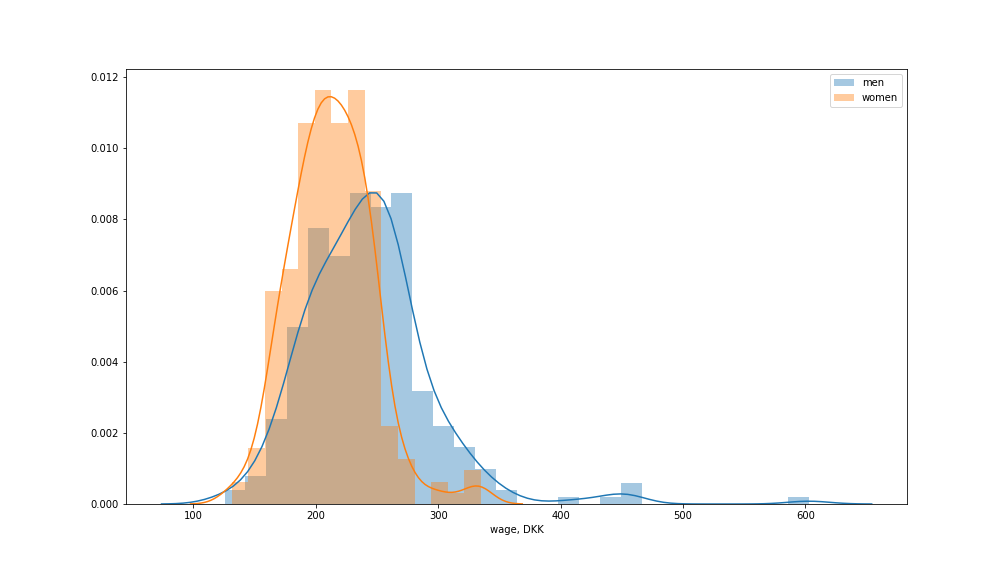
\includegraphics[scale=0.4]{figures/wage_distribution_lons20.png}
    \caption{Wage Distribution Men \& Women}
    \label{fig:my_label}
\end{figure}


\begin{figure}
    \centering
    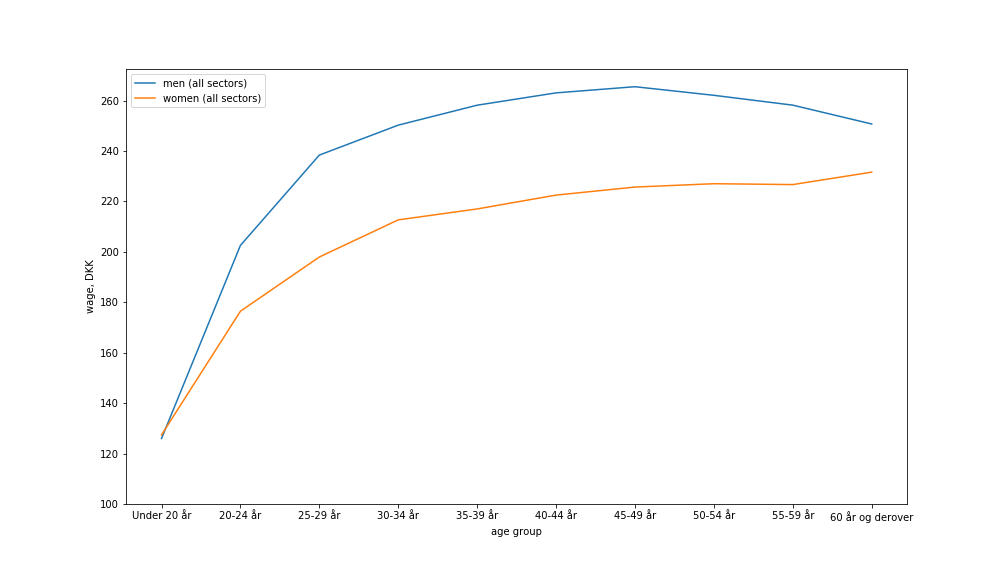
\includegraphics[scale=0.4]{figures/wage_trend_lons50.png}
    \caption{Wage Trend Men \& Women}
    \label{fig:my_label}
\end{figure}

\begin{figure}
    \centering
    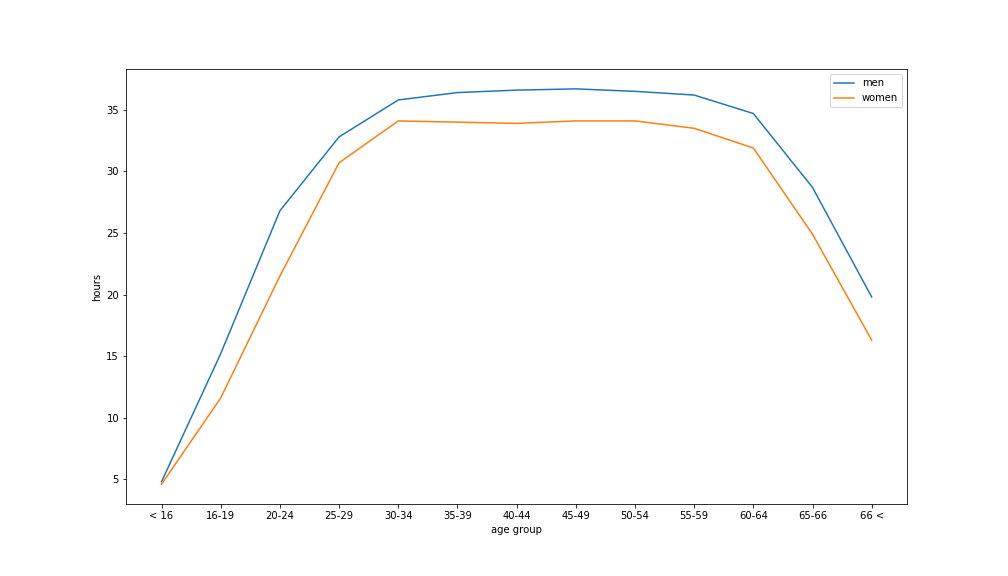
\includegraphics[scale=0.4]{figures/men_vs_women_hours_empirical.png}
    \caption{Working hours by age group (Men \& Women)}
    \label{fig:my_label}
\end{figure}